\documentclass[12pt,a4paper,oneside,czech,american]{book} % TODO: Update 'oneside' or 'twoside' - depending on number of pages

%%% TODO:
% * Create bibliography file? Can we do custom source format?
% * Create tex files for chapters - see Juriad or MAK2 essay for examples

%%% Packages:
%% Necessary packages:
\usepackage[T1]{fontenc}		% Font encoding
\usepackage[utf8]{inputenc}		% Input encoding
\usepackage[a4paper, hmarginratio=3:2]{geometry}	% Use of the A4 page and setting the margins (the binding will be wider)

%% Other packages:
% Code:
\usepackage{listings} 			 % Code formatting package

% Fonts:
\usepackage[hidelinks]{hyperref} % Hide square around URL link.
\usepackage{amsmath}  			 % Advanced mathematic package
\usepackage{color}    			 % Colorful text

% Graphics:
\usepackage{graphicx} 			 % Insert raster graphic files (PNG etc.)
\usepackage{epsfig} 			 % Insert EPS graphics files
\usepackage{float} 			  	 % Advanced figure placement options
\usepackage{caption} 			 % Captions of figure, tables, etc.

% Languages:
\usepackage{babel}

% Page formatting:
% TODO: Replace placeholder PDF with scan of orignal task paper
\usepackage{pdfpages}			 % Add PDFs into compiled PDF

% Tables:
\usepackage{tabularx}			 % Advanced table options

%%% Document settings:
% TODO: Play around with the following if the formatting of pages turns out weird
\widowpenalty=9500 	   % Completely avoid widows (last lines of paragraph on a new page)
\clubpenalty=9500 	   % Completely avoid orphans (first lines of a new paragraph on the bottom of a page)
\brokenpenalty=9500    % Prohibit page breaks after a line that has a split word at the end

\topmargin=-15mm      % Upper edge slightly smaller
\textwidth=150mm      % Text width on the page
\textheight=240mm     % Height of the text on the page

\pagenumbering{arabic} % Page numbering in Arabic numerals
\pagestyle{plain}      % Page numbering at the bottom center

\parindent=0pt 		  % Indentation of the 1st line of the paragraph
\parskip=7pt   		  % Spacing between paragraphs


%%% Custom commands:
\newcommand{\ti}{\textit} % Shortcut for cursive font
\newcommand{\tb}{\textbf} % Shortcut for bold fond


%%% Constants
\newcommand{\cvut}{České vysoké učení technické v Praze}
\newcommand{\fjfi}{Fakulta jaderná a fyzikálně inženýrská}
\newcommand{\ksi}{Katedra softwarového inženýrství}
\newcommand{\programme}{Aplikace přírodních věd}
\newcommand{\specialization}{Aplikace softwarového inženýrství}

\newcommand{\kind}{Výzkumný úkol}

\newcommand{\logoCVUT}{
\includegraphics{images/title/cvut_logo_contour_version.pdf}}

% The following was filled in accordance with the original task paper
\newcommand{\titleCZ}{Paralelní LU rozklad pro GPU}			 % Czech title of the project
\newcommand{\titleEN}{Parallel LU Decomposition for the GPU} % English title of the project
\newcommand{\paperAuthor}{Bc. Lukáš Čejka}   				 % Name and surname, including academic titles
\newcommand{\supervisor}{doc. Ing. Tomáš Oberhuber, Ph.D.} 	 % Name and surname of supervisor, including academic titles
\newcommand{\supervisorWorkspace}{\ksi, \fjfi, \cvut} 			 % Workplace of supervisor

% TODO: Can Klinkovsky be considered a consultant?
\newcommand{\consultant}{--} 								 % Consultant's name, surname and academic titles, if I have a consultant
\newcommand{\consultantWorkspace}{--} 							 % Consultant's workplace, if I have a consultant

\newcommand{\yearSubmitted}{2022}  									 % Year of handing in the thesis (not the academic years)
\newcommand{\place}{Praze} 									 % City of studying

% TODO: Fill in the following at the end
\newcommand{\keywordCZ}{Klíčová slova}   						 % Enter 5 keywords max. in Czech
\newcommand{\keywordEN}{Key words}       						 % Enter 5 keywords max. in English (translations of the Czech keywords)
\newcommand{\abstractCZ}{Popis práce česky}    				 % Abstract in Czech (roughly 7 sentences, at least 80 words)
\newcommand{\abstractEN}{Description of the project in English} % Abstract in English (translation of the Czech abstract)

% Declaration in Czech
\newcommand{\declarationCZ}{Prohlašuji, že jsem svůj výzkumný úkol vypracoval samostatně a použil jsem pouze podklady (literaturu, projekty, SW atd.) uvedené v přiloženém seznamu.}

% Declaration in English
\newcommand{\declarationEN}{I declare that I have carried out my research project independently and I have used only the materials (literature, projects, software, etc.) listed in the bibliography.}

% Acknowledgement in Czech
\newcommand{\acknowledgementCZ}{Chtěl bych poděkovat doc. Ing. Tomáš Oberhuber, Ph.D. za vedení mé práce a za podnětné návrhy, které ji obohatily.}

% Acknowledgement in English (translation of the Czech acknowledgement)
\newcommand{\acknowledgementEN}{I would like to thank doc. Ing. Tomas Oberhuber, Ph.D. for supervising my project and for the inspiring proposals that enriched it.}




\begin{document}
\shorthandoff{-} % This disables the issues with the 'czech' package: https://tex.stackexchange.com/questions/477449/incomplete-iffalse-related-listlisting-textit-and-textcolor




%%%%%%%%%%%% TITLE PAGE %%%%%%%%%%%%
\thispagestyle{empty}
\selectlanguage{czech}%

\begin{center}
	{\LARGE
		\cvut\par
		\fjfi
	}
    \vspace{10mm}

    \begin{tabular}{c}
		\tb{\ksi} \\[3pt]   
		\tb{Obor: \specialization}\\
    \end{tabular}

   \vspace{10mm} \logoCVUT \vspace{15mm} 

   {\huge \tb{\titleCZ}\par}
   \vspace{5mm}
   \selectlanguage{american}%
   {\huge \tb{\titleEN}\par}
   \selectlanguage{czech}%
   
   \vspace{15mm}
   {\Large \MakeUppercase{\kind}}

   \vfill
   {\large
    \begin{tabular}{ll}
    Vypracoval: & \paperAuthor\\
    Vedoucí práce: & \supervisor\\
    Rok: & \yearSubmitted
    \end{tabular}
   }
\end{center}

\clearpage{\pagestyle{empty}\cleardoublepage} % prázdná stránka za tou "titulní", bez čísla




%%%%%%%%%%%% TASK PAPER %%%%%%%%%%%%
% TODO: Include the orginal scanned paper - signed by my supervisor and the department head
% TODO: Before binding, one of the printed copies of this paper should CONTAIN THE ORIGINAL SIGNED PAPER
\newpage  			  % DO NOT TOUCH!
\thispagestyle{empty} % DO NOT TOUCH!

% Task paper scanned as a 2-page PDF:
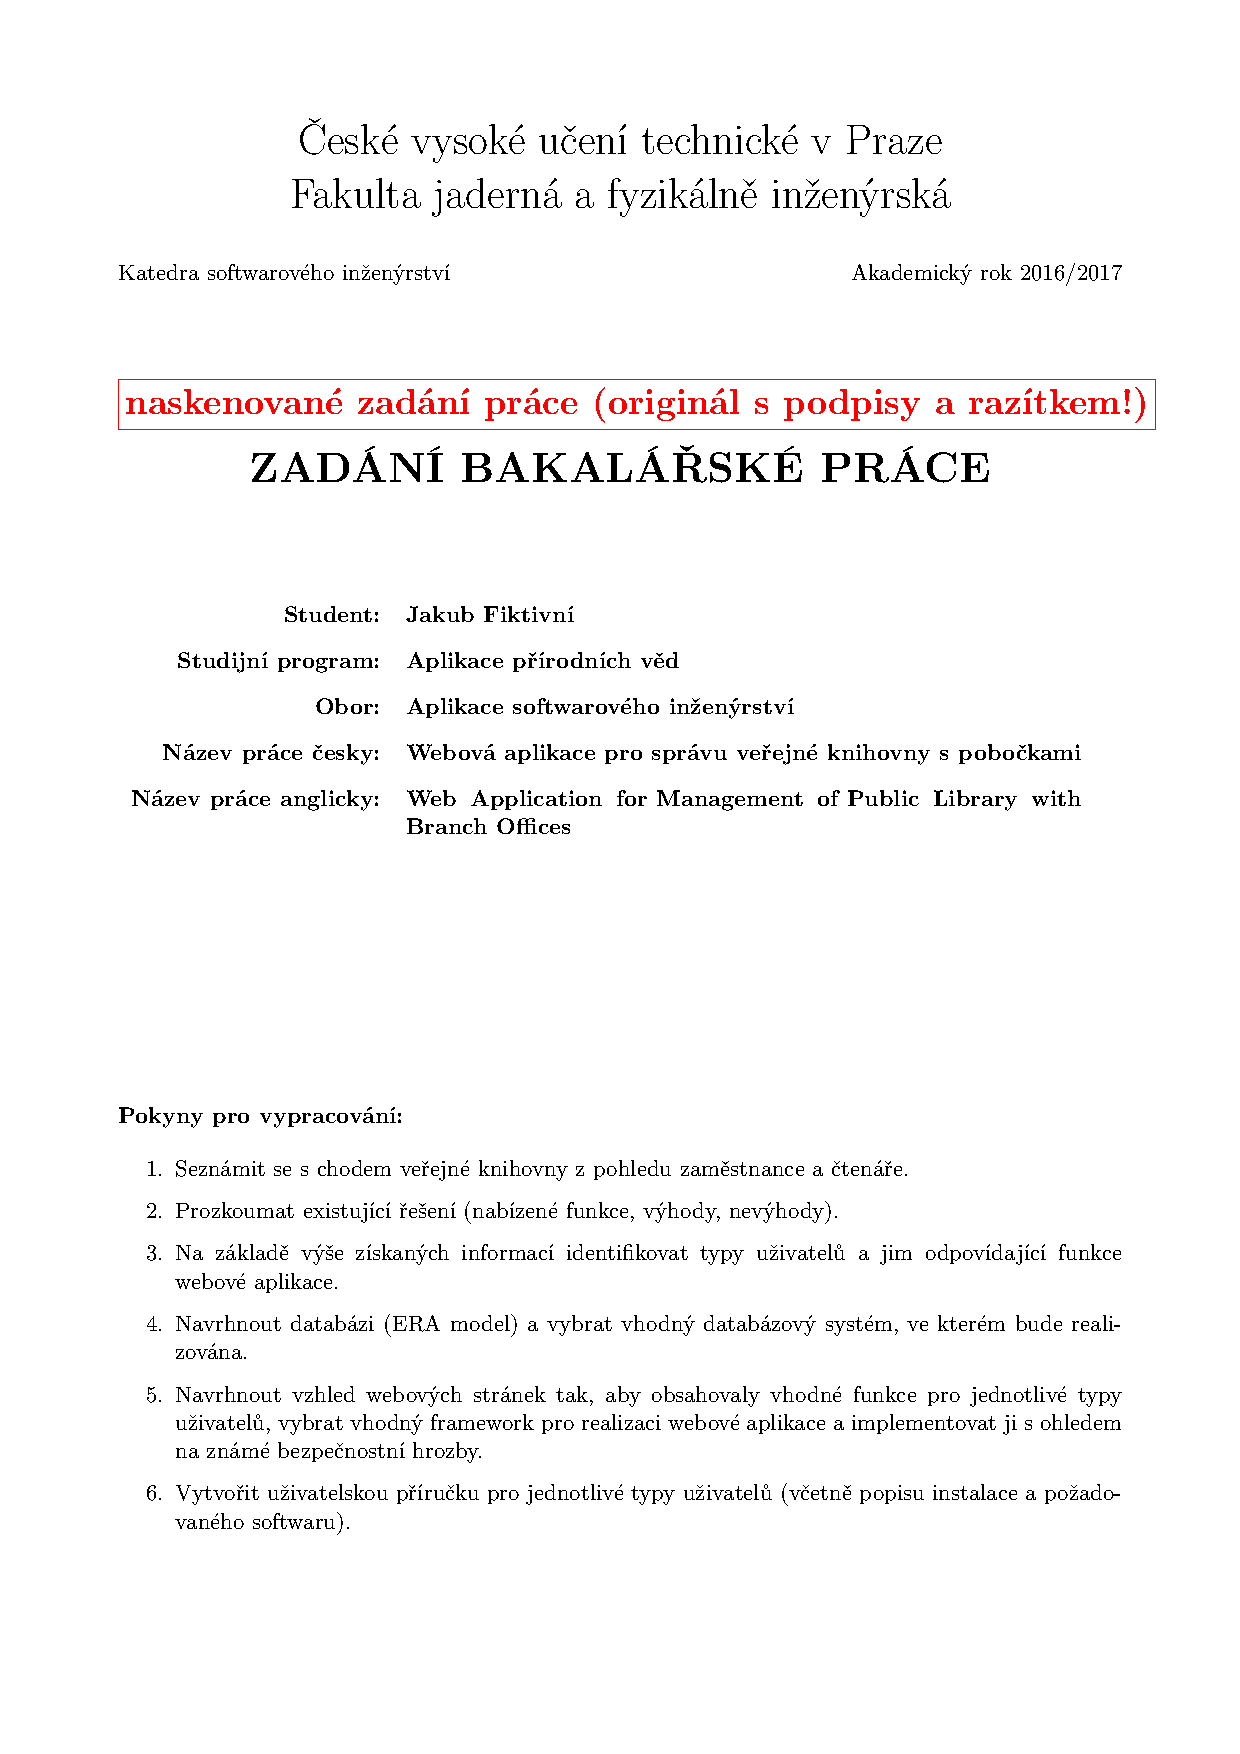
\includepdf[pages={1,2}]{resources/zadani_cele.pdf} % TODO: Replace with the correct paper




%%%%%%%%%%%% DECLARATION %%%%%%%%%%%%
\newpage 			  % DO NOT TOUCH!
\thispagestyle{empty} % DO NOT TOUCH!

~ 					  % DO NOT TOUCH!
\vfill 				  % Empty fill. DO NOT TOUCH!

\tb{Prohlášení} 	  % DO NOT TOUCH!

\vspace{1em} 		  % Vertical space. % DO NOT TOUCH!
\declarationCZ

\selectlanguage{american}%
\vspace{1em}
\tb{Declaration}

\vspace{1em}
\declarationEN
\selectlanguage{czech}%

\vspace{2em}  									 							  % DO NOT TOUCH!
\hspace{-0.5em}\begin{tabularx}{\textwidth}{X c} 							  % DO NOT TOUCH!
V \place\ dne .................... &........................................ \\ % DO NOT TOUCH!
	& \paperAuthor
\end{tabularx} % DO NOT TOUCH!




%%%%%%%%%%%% ACKNOWLEDGEMENT  %%%%%%%%%%%%
\newpage
\thispagestyle{empty}

~
\vfill % Empty fill

\tb{Poděkování}

\vspace{1em} % Vertical space. % DO NOT TOUCH!
\acknowledgementCZ

\selectlanguage{american}%
\vspace{1em}
\tb{Acknowledgment}

\selectlanguage{czech}%
\vspace{1em} % Vertical space. % DO NOT TOUCH!
\acknowledgementEN
\begin{flushright}
\paperAuthor
\end{flushright}  % Acknowledgement page ends here




%%%%%%%%%%%% ABSTRACT %%%%%%%%%%%% 
\newpage   			  % DO NOT TOUCH!
\thispagestyle{empty} % DO NOT TOUCH!

% Preparation: DO NOT TOUCH the next 8 lines!
\newbox\odstavecbox
\newlength\vyskaodstavce
\newcommand\odstavec[2]{%
    \setbox\odstavecbox=\hbox{%
         \parbox[t]{#1}{#2\vrule width 0pt depth 4pt}}%
    \global\vyskaodstavce=\dp\odstavecbox
    \box\odstavecbox}
\newcommand{\delka}{120mm} % Text width in 2nd table column

% Using the preparation: DO NOT TOUCH commands inside the "tabular" section!
\begin{tabular}{ll}
  {\em Název práce:} & ~ \\
  \multicolumn{2}{l}{\odstavec{\textwidth}{\bf \titleCZ}} \\[1em]
  {\em Autor:} & \paperAuthor \\[1em]
  {\em Studijní program:} & \programme \\
  {\em Obor:} & \specialization \\
  {\em Druh práce:} & \kind \\[1em]
  {\em Vedoucí práce:} & \odstavec{\delka}{\supervisor\\ \supervisorWorkspace} \\
  {\em Konzultant:} & -- %\odstavec{\delka}{\consultant \\ \consultantWorkspace}  % TODO: Remove the text "-- %" if you had a consultant
 \\[1em]  
  \multicolumn{2}{l}{\odstavec{\textwidth}{{\em Abstrakt:} ~ \abstractCZ  }} \\[1em]
  {\em Klíčová slova:} & \odstavec{\delka}{\keywordCZ} \\[2em]
  \selectlanguage{american}%
  {\em Title:} & ~\\
  \multicolumn{2}{l}{\odstavec{\textwidth}{\bf \titleEN}}\\[1em]
  {\em Author:} & \paperAuthor \\[1em]
  \multicolumn{2}{l}{\odstavec{\textwidth}{{\em Abstract:} ~ \abstractEN  }} \\[1em]
  {\em Key words:} & \odstavec{\delka}{\keywordEN}
\end{tabular}




%%%%%%%%%%%% CONTENTS OF THE PAPER %%%%%%%%%%%%
\selectlanguage{american}%
\newpage  		 % DO NOT TOUCH!
\parskip=0pt
\tableofcontents % DO NOT TOUCH!
\parskip=7pt
\newpage 		 % DO NOT TOUCH!




%--------------------------------------------------------
%|         The PAPER ITSELF begins here                 |
%--------------------------------------------------------

\chapter*{Introduction}				 		 % DO NOT TOUCH!
\addcontentsline{toc}{chapter}{Introduction} % DO NOT TOUCH!

Put my introduction text here (1-3 pages, do not divide it into sub-pages) or insert it from a separate file using: \texttt{\textbackslash input\{introduction.tex\}}.
% TODO: If the input file includes the command "\chapter{...}" then remove the one a few lines above



\chapter{Title of first chapter}
Put the text of your first chapter here, or insert it from a separate file using: \texttt{\textbackslash input\{chpater\_one.tex\}}.
% TODO: If the input file includes the command "\chapter{...}" then remove the one a few lines above




\chapter*{Conclusion} % DO NOT TOUCH!
\addcontentsline{toc}{chapter}{Conclusion} % DO NOT TOUCH!

Put my conclusion text here (1-3 pages, do not divide it into sub-pages) or insert it from a separate file using: \texttt{\textbackslash input\{conclusion.tex\}}.




%%%%%%%%%%%% BIBLIOGRAPHY %%%%%%%%%%%%
\clearpage  							   	 % DO NOT TOUCH!
\addcontentsline{toc}{chapter}{Bibliography} % DO NOT TOUCH!

\begin{thebibliography}{3}
	% Format: ČSN ISO 690. It can be generate using http://www.citacepro.com - it can generate TeX
	% Ordering: Alphabetical according to author (from the first word if the author is not known)
	% \bibitem{link} Author. \ti{Title of item}. City. Publisher. Year.
	\bibitem{Sharma2019}
	SHARMA, Bharatkumar a Jaegeun HAN. \textit{Learn CUDA Programming: A beginner's guide to GPU programming and parallel computing with CUDA 10.x and C/C++}. Birmingham: Packt Publishing, 2019. ISBN 978-1788996242.
	\bibitem{Saad2003}
	SAAD, Y. \textit{Iterative methods for sparse linear systems}. 2nd ed. Philadelphia: Society for Industrial and Applied Mathematics, 2003. ISBN 978-0898715347.
	\bibitem{Anzt2019}
	ANZT, Hartwig, Tobias RIBIZEL, Goran FLEGAR, Edmond CHOW a Jack DONGARRA. \ti{ParILUT - A Parallel Threshold ILU for GPUs}. In: 2019 IEEE International Parallel and Distributed Processing Symposium (IPDPS) [online]. IEEE, 2019, 2019, s.~231-241 [cit. 2021-03-16]. ISBN 978-1-7281-1246-6. Dostupné z: doi:10.1109/IPDPS.2019.00033
	
\end{thebibliography}




%%%%%%%%%%%% WORK ATTACHMENTS %%%%%%%%%%%%
\newpage 									% DO NOT TOUCH!
\addcontentsline{toc}{chapter}{Attachments}	% DO NOT TOUCH!
\appendix 								 	% DO NOT TOUCH!


%%%%%%%%%%%% Attachment A (1st chapter in terms of attachments) %%%%%%%%%%%%

\chapter{Title of first attachment}
Write the text for your first attachment here, or insert it using: \texttt{\textbackslash input\{attachment\_A.tex\}}.
% TODO: If the input file includes the command "\chapter{...}" then remove the one a few lines above




\end{document}
